\chapter{Machine learning}\label{machineLearning}

The chapter briefly explains the theory of \textbf{supervised learning} focusing in the context of regression with Gaussian processes. It theoretically introduces the statistical model that will be used to produce results related to the Windkessel model seen in the chapter \ref{windkessel}.\\
The sources used for the drafting of the chapter are: \cite{murphy_probabilistic_2022}, \cite{wiki:datasets}, \cite{wiki:overfitting}, \cite{pytorch:R2score}, \cite{wang_intuitive_2022}, \cite{noauthor_tutorial_nodate}, \cite{murphy_machine_2012}, \cite{gelman_bayesian_1995}, \cite{wiki:gradientDescend}, \cite{ruder_2022}, \cite{kingma_adam_2017}, \cite{JMLR:v12:duchi11a}, \cite{bottou2012stochastic}.


\begin{textblock*}{0.64\textwidth}(3.5cm+0.36\textwidth,18.5cm)
\epigraph{Il sole è sorto e tramontato per miliardi di anni. Il sole è tramontato anche stanotte. Con un'elevata probabilità, il sole domani sorgerà. Ma questo numero è molto più grande per colui che, vedendo nella totalità dei fenomeni il principio che regola i giorni e le stagioni, si rende conto che nulla al momento attuale può arrestarne il corso.}{Pierre Simon Laplace}
\end{textblock*}

\newpage

\section{Introduction to machine learning}
Machine learning is a branch of artificial intelligence, a discipline that studies the theoretical foundations and techniques that enable the design of systems capable of providing computers with performances that would seem to be the exclusive domain of human intelligence.\\
Of this vast branch, the work is only interested in regression problems, as opposed to classification problems.

In more practical terms, the main purpose of machine learning is the study and construction of algorithms that can learn to make predictions about data. Such algorithms work by relying on decisions guided by the dataset through the construction of a mathematical model.\\
A specific type of learning is used in this work, which is the \textit{supervised} learning.

\begin{defi}[Supervised learning]
    \textbf{Supervised learning} is a machine learning technique that aims to instruct a computer system to make predictions based on a series of examples consisting of input and output pairs.
\end{defi}

\section{Dataset}\label{dataset}

Per ottimizzare la costruzione di algoritmi predittivi, i dati di input vengono divisi in più set di dati con ruoli diversi. Tipicamente viene usata una specifica partizione dei dati in tre dataset: \textbf{training}, \textbf{validation} e \textbf{test set}.


\begin{defi}[Training set]
Il \textbf{training set} è un insieme di esempi utilizzati durante il processo di apprendimento per determinare (o imparare) le combinazioni ottimali di parametri.
\end{defi}

In pratica, è sui dati del training set che viene eseguito il metodo di ottimizzazione scelto, aggiornando quindi i valori dei parametri o degli iperparametri.

\begin{defi}[Validation set]
Il \textbf{validation set} è un set indipendente di dati usato per valutare il modello addestrato sul training set.
\end{defi}
La valutazione (o \textit{validazione}) del modello sul validation set porta a decidere quali siano i migliori valori per i parametri (o iperparametri) in base alla performance sul validation set, appunto. Nel caso dell'elaborato viene usato un early-stopper, che sceglie come miglior modello quello con minore errore subito prima che si verifichi overfitting.

\begin{defi}[Test set]
Un \textbf{test set} è un set indipendente di dati dal training set  usato solo per valutare le prestazioni del modello.
\end{defi}

\newpage

Cioè il test set viene usato per valutare su un terzo set di dati indipendente il modello scelto in base alla performance sul validation set. Si ottengono così caratteristiche di prestazione come la precisione, la sensibilità, la specificità... Questo dataset è importante perché permette di valutare la performance del modello su un terzo insieme di dati indipendente dai precedenti evitando il rischio di overfitting: se un modello addestrato sul training test si adatta anche al test set, si è verificato un overfitting minimo.

È stato più volte citato il problema dell'\textbf{overfitting}, viene quindi riportata la definizione.

\begin{defi}[Overfitting]
L'\textbf{overfitting} è la generazione di un modello (o un'analisi) che corrisponde troppo strettamente a un particolare insieme di dati e può quindi non riuscire a prevedere osservazioni future in modo affidabile.
\end{defi}

L'overfitting può verificarsi per esempio includendo troppi parametri regolabili o usando un approccio troppo complicato, come mostrato in figura \ref{overfittigComplex}. Chiaramente, quando si confrontano diversi tipi di modelli la complessità deve tenere conto dell'influenza di ogni parametro sull'output\footnote{Si noti che si può incorrere nel problema opposto usando un approccio troppo semplice: l'underfitting. Ad esempio cercando di approssimare con una regressione lineare un campione con un andamento parabolico.}.

\begin{figure}[htbp]
    \centering
    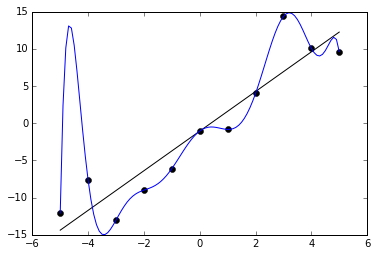
\includegraphics[width=0.6\textwidth]{images/Machine learning/Overfitted_Data.png}
    \caption{Esempio di overfitting. I dati (approssimativamente lineari) sono approssimati da una funzione lineare e da una polinomiale. Anche se la funzione polinomiale fornisce un adattamento quasi perfetto, ci si può aspettare che la funzione lineare generalizzi meglio i dati. \cite{wiki:overfitting}}
    \label{overfittigComplex}
\end{figure}

\newpage

L'overfitting è particolarmente probabile nei casi in cui l'apprendimento è stato eseguito troppo a lungo o in cui ci sono pochi dati per l'apprendimento, facendo sì che il modello si adatti a caratteristiche casuali molto specifiche dei dati di formazione che non hanno alcuna relazione causale con l'output. In questo caso di overfitting, la performance sul training set continua ad aumentare mentre la performance sul validation set peggiora, come mostrato in figura \ref{overfittingError}.



\begin{figure}[htbp]
    \centering
    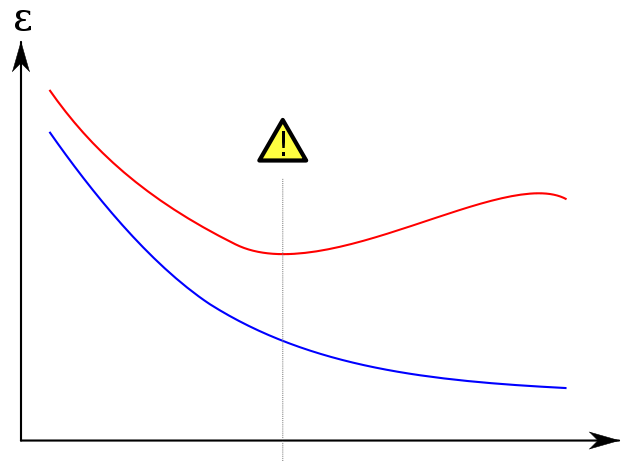
\includegraphics[width=0.6\textwidth]{images/Machine learning/Overfitting error.png}
    \caption{Overfitting nell'apprendimento supervisionato. Il training error (errore sul training set) è mostrato in blu, il validation error (errore su validation set) in rosso, entrambi in funzione del numero di cicli di training. \cite{wiki:overfitting}}
    \label{overfittingError}
\end{figure}


\subsection{Loss function}
Finora è stato delineato il problema che interessa l'elaborato: cercare una funzione $f$ per predire l'output $Y$ a partire dai valori dell'input $X$. Per farlo è necessaria una funzione di perdita, in inglese \textit{loss function}, $L(Y, f (X))$ per penalizzare gli errori di previsione.

\begin{defi}[Loss function]
Una \textbf{loss function} è una funzione in forma $\mathcal{L}(y_{\text{true}},y_{ \text{guess}})$ che definisce la perdita subita (o l'errore commesso) predicendo il valore $y_\text{guess}$ quando il valore vero è $y_{\text{true}}$,  fornendo quindi una valutazione delle capacità predittive del modello.
\end{defi}

Sarà questa la funzione da minimizzare con un algoritmo di ottimizzazione per l'adattamento degli iperparametri del processo gaussiano. Evidentemente la scelta della loss function dipende dal contesto.

%\section{Mean squared error}
%Per gli scopi dell'elaborato, si farà uso del \textit{mean squared error}.

%\begin{defi}[Mean squared error]
%Il \textbf{mean squared error} (o \textit{MSE}) è una \textit{loss function} definita come:
%\[
%\frac{1}{n}\sum^{n}_{i=1}(Y_i-f(X_i))^2,
%\]
%dove su $n$ dati raccolti, $Y_i$ sono gli output reali, $f(X_i)$ sono gli output predetti a partire da $X_i$.
%Poiché deriva dal quadrato della distanza euclidea, è sempre un valore positivo che diminuisce man mano che l'errore si avvicina a zero.
%\end{defi}
%Verrà usato non come loss function, ma per monitorare l'andamento del training.


%\section{Coefficiente di determinazione}
%Il coefficiente di determinazione fornisce una misura della bontà di adattamento di un modello, cioè quanto le previsioni di regressione approssimano i punti dei dati reali. Varia tra 0 e 1\footnote{Si possono apportare modifiche al coefficiente per fargli assumere anche altri valori, ma non vengono applicate nell'elaborato}, un $R^2$ di 1 indica che le previsioni di regressione si adattano perfettamente ai dati.

%Poichè il coefficiente di determinazione varia in un intervallo unitario, può essere più (intuitivamente) informativo di altre misure di errore (come il mean absolute error o il mean squared error) poiché tendono ad assumere valori su intervalli arbitrari oppure ad esprimere una percentuale.

%\begin{defi}[Coefficiente di determinazione]
%Date $y_i$ le osservazioni, $\overline{y}$ la media delle osservazioni, $\hat{y}_i$ i dati predetti dal modello:
%\[
%R^2 = 1-\frac{\sum_{i=1}^{n}(y_i-\hat{y}_i)}{\sum_{%i=1}^{n}(y_i-\overline{y})}
%\]
%\end{defi}
%Si noti che questo coefficiente non indica se:
%\begin{itemize}
%    \item una variabile sia statisticamente %significativa;
%    \item è stata usata la regressione corretta;
%    \item è stato scelto l'insieme più appropriato %di variabili indipendenti;
%    \item ci sono abbastanza dati per trarre una %conclusione solida.
%\end{itemize}

%Si noti inoltre che $R^2$ è una versione riscalata del mean squared error più facile da interpretare in quanto non dipende dalla scala dei dati.

\newpage
\section{Parametric and non-parametric models}
There is an important distinction to be made about statistical models: parametric and non-parametric models. The type of model, in fact, greatly modifies the theoretical approach to be used and thus the application results. 


\subsection{Parametric models}
Parametric models assume that the distribution of data can be modelled in terms of a finite set of parameters.\\
A classic example is regression in which, given observations, an attempt is made to estimate a possible functional relationship existing between the dependent variable and the independent variables. If we assume a linear regression model, where the relationship is expressed by the function $f(x) = \theta_1 + \theta_2x$ where $x$ is the input data, we need to find the values of the parameters $\theta_1$ and $\theta_2$ to define $f$. In many cases, the assumption of the linear model is not sufficient, and a polynomial model (with more parameters) is needed: $f(x) = \theta_1+\theta_2x+\theta_3x^2$.\\
Thus given a dataset $D$ with $n$ observed points, after the process of \textit{training} we assume that all information about the functional relationship has been captured by the parameters $\theta_i$.  When running regressions using parametric models, the complexity and flexibility of the models is limited by the number of parameters. 

\subsection{Non-parametric models}
Contrary to what one might think, a \textbf{non-parametric model} is not a model without parameters. \\
Intuitively, if the number of parameters of a model increases with the size of the observed dataset, it is a non-parametric model. Theoretically, this allows the model to have infinite parameters and thus not depend on a rigid function structure $f$, increasing its flexibility.\\
Of interest in the paper is regression using Gaussian processes, which follows a non-parametric Bayesian approach (seen in \ref{regressioneGP}). It is capable of \textit{learning} a wide variety of input-output relationships using a theoretically infinite number of parameters and letting the data determine the level of complexity through the means of Bayesian inference.

See \ref{gerarchica} for a clarification of the difference between parameters and hyperparameters in regression using Gaussian processes.

\newpage

\subsection{Hierarchical structure}\label{gerarchica}
It is common to use a hierarchical structure of parameters and hyperparameters in regression models.

The parameters reside at the lowest level. For example, in the case of linear regression, the parameters are the $\theta_i$, or in the case of a neural network model the weights associated with the neurons.\\
At the second level are the \textit{iperparameters} that control the distribution of parameters at the lower level and thus whose value is used to control the learning process.\\

In the case of Gaussian processes, since they are a non-parametric model, it is not obvious what the parameters of the model are. One can take the values of the (noise-free) function evaluated on the observed data as parameters. Then let $X=\{(x_i,y_i): i\in I\}$ be the set of observed data, the elements $y_i$ can be considered the parameters of the model. Obviously, the larger $X$, the more parameters there are. In practical terms, it was seen in \ref{regressioneGP} how the observed data correspond to the information about the shape of the function, thus how the accuracy depends on the number of observed data.

It is also possible to give a different interpretation of the model parameters using a different theoretical interpretation (\textit{weight-space view}), which has not been introduced in the paper.\footnote{Further: \cite{rasmussen_gaussian_2006}}\\

The hyperparameters, on the other hand, are the parameters of the mean function and the kernel function. Pragmatically, to do regression, it is necessary to work on the estimation of the hyperparameters.


\newpage


\section{Optimisation of hyperparameters}

\subsection{Bayesian inference}
Bayesian inference is a method of statistical inference in which Bayes' theorem is used to update the probability of a hypothesis as more information becomes available. 

The Bayesian process of data analysis can be idealised by dividing it into the following three stages:
\begin{enumerate}
    \item Creation of a complete probability model\\
    The model consists of a joint probability distribution for all quantities related to the problem and must be consistent with the knowledge of the underlying scientific problem.
    \item Conditioning of observed data\\ The appropriate a posteriori distribution, i.e. the probability distribution of the unobserved quantities conditioned on the observed data, is calculated and interpreted.
    \item Evaluation of model fit\\
    It is assessed how well the model fits the data and whether the substantive conclusions are reasonable. At this stage, it is possible to modify or expand the model and repeat the three steps.
\end{enumerate}
The Bayesian approach can be interpreted as a formalisation of the scientific method, in which an attempt is made to update scientific knowledge through experiments and observations.\\
Moreover, this statistical approach is flexible enough to be used in complex problems, even those with many parameters.\\

In the area of Gaussian processes, the use of Bayesian inference in the optimisation of hyperparameters is studied.

\newpage

\subsection{Bayes' Theorem}
\begin{teo}[Bayes' Theorem]
    Let $A, B$ be events, let $\probP(B)\neq 0$, then:
\[
\probP(A|B) = \frac{\probP(B|A)\probP(A)}{\probP(B)}.
\]
\end{teo}
\begin{proof}
    From the definition of conditional probability we have: $\probP(A\cap B) = \probP(A|B)\probP(B)$, from which it follows $\probP(A|B)=\frac{\probP(A\cap B)}{\probP(B)}$ if $\probP(B)\neq 0$; similarly: $\probP(B|A)=\frac{\probP(A\cap B)}{\probP(A)}$ if $\probP(A)\neq 0$. Substituting $\probP(A\cap B)$ into the expression of $\probP(A|B)$ concludes.
\end{proof}

\vspace{0.5cm}

In the Bayesian context, the purpose of analysing a model is to draw statistical conclusions about a parameter $\theta$ (or similarly about a vector of parameters\footnote{For the moment, the case of parameters is considered, but what is said immediately extends to the case of hyperparameters, as seen in \ref{evidenzaBayesiana}}) or about unobserved data; these conclusions are formulated in terms of probabilities conditional on the observed value of $y$. 
In order to make probability statements on $\theta$ observed $y$ data, it is necessary to start with a model that provides a joint probability distribution for $\theta$ and $y$, which can be factored into two components: $\probP(\theta)$, i.e. the a priori distribution describing the knowledge about the distribution of $\theta$ before observing the data, and $\probP(y|\theta)$, i.e. the data (or sample) distribution:
\[
\probP(\theta, y)=\probP(\theta)\probP(y|\theta).
\]

Applying Bayes' theorem we obtain the \textit{a posteriori distribution}:
\[
\probP(\theta | y)=\frac{\probP(\theta)\probP(y|\theta)}{\probP(y)},
\]
in which the denominator can be rewritten, by the absolute probability theorem (\textit{law of total probability}), as:
\[
\probP(y)=\begin{cases}\sum_\theta \probP(\theta)\probP(y| \theta)\\\int\probP(\theta)\probP(y| \theta)d\theta \end{cases} \text{ in base a }\theta.
\]
Since $\probP(y)$ does not depend on $\theta$ and fixing $y$ it is possible to rewrite the a posteriori distribution as:

\[
\probP(\theta | y)\propto \probP(\theta)\probP(y|\theta),
\]
where, having fixed $y$, $\probP(y|\theta)$ is a function of $\theta$.

\newpage

\subsection{Bayesian evidence}\label{evidenzaBayesiana}
In the context of statistical models, the reinterpretation of Bayes' theorem (and what was said in the previous section) is:
\[
\probP(\theta | X, \alpha) = \frac{\probP(X|\theta, \alpha)\probP(\theta | \alpha)}{\probP(X|\alpha)}\propto \probP(\theta | \alpha) \probP(X|\theta, \alpha),
\]
where: $\theta$ is the vector of parameters, $\alpha$ the vector of hyperparameters, $X$ the sample of observed data. In this case the a priori distribution is $\probP(\theta|\alpha)$\footnote{ Note that it is conditional on the value of the hyperparameters. This is due to the definition of the hyperparameters, which control the distribution of the parameters, as mentioned in \ref{gerarchica}. }, the distribution of the parameters before observing the data $X$; $\probP(X|\theta)$, the sample distribution which is the distribution of the observed data conditional on the value of the parameters; and $\probP(X|\alpha)$, the \textbf{evidence} (also called \textit{marginal likelihood}) which is the distribution of the data conditional on the hyperparameters. The latter can be rewritten as
\[
\probP(X|\alpha) = \int \probP(X|\theta)\probP(\theta | \alpha)d\theta,
\]
i.e. as the distribution of marginalised data on the parameters.

In addition to being the normalisation term in Bayes' theorem, another possible way of interpreting marginal likelihood is to consider it the probability of having generated the (observed) dataset $X$ given the hyperparameters $\alpha$.

Using Bayes' theorem again, we obtain:
\[
\probP(\alpha |X) = \frac{\probP(X|\alpha)\probP(\alpha)}{\probP(X)}\propto \probP(X|\alpha) \probP(\alpha),
\]
i.e. the a posteriori distribution (representing the distribution of the observed hyperparameters of the $X$ data) is proportional to the marginal likelihood. Since in the case considered by the paper, i.e. Gaussian processes, one of the objectives is to find the distribution of the hyperparameters (i.e. the form of the covariance function, in other words $\probP(\alpha|X)$)), the approach adopted is to maximise the marginal likelihood, taking advantage of the dependence highlighted in the previous formula. This approach is called the \textbf{evidence approach}.

\newpage

\subsection{Alternatives to Bayesian evidence}
The choice of approach for estimating the value of parameters or hyper-parameters depends very much on the situation. For example:
\begin{itemize}
    \item Maximising the \textit{likelihood}:
    one maximises $L(\alpha, \theta | X)$ (the likelihood function), thus finding values of $\alpha$ and $\theta$ that maximise it;
    \item Partial maximisation of \textit{likelihood}:
    Given the case in which $L(\alpha, \theta |X)=L_1(\alpha | X)L_2(\theta|X)$, only the factor of interest is maximised, in the present case $L_1(\alpha | X)$ is maximised;
    \item Maximising the \textit{marginal likelihood}:
    marginalises on $\theta$, then maximises $\probP(X|\alpha)$ which depends only on $\alpha$.
\end{itemize}
The paper applies the last case since the necessary calculations are all analytically solvable. In other situations, this approach requires a numerical approximation which may lead to stability problems, which is why it is not always an approach used.




\subsection{In Gaussian processes}\label{neiProcessiGaussiani}
The approach that Gaussian processes follow is to define a \textit{distribution over functions}, update it from observed data and use it to make predictions on new inputs. \\
Consider what was done in the section \ref{noisyPrediction}: an a priori distribution was defined on the functions, which was then converted into an a posteriori distribution by updating the information thanks to the observed data. Unlike the \textit{noise-free} case, however, one does not obtain a function that perfectly interpolates the data. In this case, it is therefore necessary to choose appropriate hyperparameters in order to optimise the form of the function: this estimation is done by means of an evidence approach, taking advantage of the fact that the expressions of the integrals are all analytically solvable.\\


In this case, the marginal likelihood is:
\[
\probP(\bf{y}|\bf{\alpha}) = \int \probP(\bf{y}| \mathbf{f},\bf{\alpha})\probP(\mathbf{f}|\bf{\alpha}) d\mathbf{f},
\]

where $\bf{\alpha}$ are the hyperparameters, $\mathbf{f}$ are observed data without error (they are the parameters), $\bf{y}$ are the observed data.\\
Note that $\probP(\mathbf{f}|\bf{\alpha})$ is the a priori distribution of the error-free function and is a multivariate Gaussian distribution since $\mathbf{f}|\alpha\sim \mathcal{N}(m, K)$ with $K$ the Gram matrix of the covariance function and $m$ the evaluation of the mean function on the input vector. Furthermore, from the definition of $\mathbf{y}$ we have $\mathbf{y}|\mathbf{f}\sim \mathcal{N}(\mathbf{f}, \sigma_n^2I)$, where $\epsilon\sim \mathcal{N}(0,\sigma_n^2)$.

\newpage

The calculations reported in \cite{rasmussen_gaussian_2006} conclude:
\[
L=\text{log}(\probP(\mathbf{y}|\alpha))=-\frac{1}{2}\text{log}(|K+\sigma_n^2I|)-\frac{1}{2}(\mathbf{y}-m)^{\text{T}}(K+\sigma_n^2I)^{-1}(\mathbf{y}-m)-\frac{n}{2}\text{log}(2\pi)
\]

The same result can be obtained by avoiding analytical accounts by noting: $\mathbf{y}\sim \mathcal{N}(m, K+\sigma_n^2I)$. At this point, it is easy to calculate the partial derivatives with respect to the hyperparameters of the covariance function and the mean function. This is of fundamental importance for numerical optimisation methods.

Note that marginal likelihood maximisation is preferable to likelihood maximisation (or other likelihood methods) because with other forms of likelihood overfitting can be achieved (see \ref{dataset} for the definition of overfitting). In contrast, marginal likelihood does not perform \textit{fitting} of function values, but rather integrates (marginalises) them, i.e. technically it cannot do overfitting because no \textit{fit} occurs. \\

For further considerations, account details and insights on how to optimise numerical calculations, see \cite{rasmussen_gaussian_2006}.




\section{Optimisation method}
Optimisation is the branch of mathematics that studies theory and methods for finding the maximum and minimum points of a function. This section aims to retrace the main theoretical steps that led to the construction of the optimisation method later used in marginal likelihood maximisation: Adam.

\subsection{Form of the function to be optimised}\label{costfunction}
In order to understand the difference between the optimisation methods shown, it is important to understand the form of the function to be optimised.
In supervised learning, we have a dataset of observations that we want to learn from. To do this, in short, we define a function that represents the error that our model makes on the dataset of observed values\footnote{See the section \ref{dataset}, where we explain how to divide a dataset into subsets with different roles.}: the goal is to minimise this function, and to do this, it is necessary, using an appropriate algorithm, to change the values of the parameters (in the case under consideration, a non-parametric model, the hyperparameters are changed).

\newpage

Since the observed dataset will potentially contain a lot of data, it is necessary to take into account the error committed by evaluating it in each observed dataset. Generally, the error function has a form:
\[
Q(w)=\sum_{i=1}^{n}Q_i(w),
\]
where each addend tends to depend on a single datum in the input dataset. An example is:
\[
f(m,b)=\sum_{i=1}^{N}(y_i-(mx_i+b))^2,
\]
i.e. the method of least squares in linear regression.\\
Note that in the present case, the function to be optimised, the marginal likelihood, is a sum in which the $i$-th addend does not depend only on the $i$-th observed data.


\subsection{Learning rate}
The iterative optimisation methods have a similar form: given $\theta_0$ initial point, each iteration updates the point as:
\[
\theta_{t+1}=\theta_t+\eta_td_t,
\]
where $d_t$ represents a direction and is defined according to the method, $\eta_t$ is the step length (\textit{step size}) or \textit{learning rate} and indicates by how much one moves in the direction $d_t$. The learning rate can be constant or can be updated every iteration.


\newpage

\subsection{Gradient method \cite{ruder_2022}}
The \textbf{gradient method} exploits the fact that the gradient is the direction of maximum growth of the function. It has a form:
\begin{align*}
    &\text{Given an initial value }\omega_0, \eta_0\\
    &\text{To be repeated until an approximation of the minimum is found:}\\
    &\quad \omega_{k+1}=\omega_k - \eta_k\cdot \nabla Q(\omega_k).
\end{align*}
By "\textit{Repeat until an approximation of the minimum is found}" is meant that the method is repeated until an output condition is met that incorporates the precision required of the approximation.\\
Since, as seen in \ref{costfunction}, it is necessary to evaluate the gradient on each element of the dataset, it can be an onerous method, especially in terms of memory.\\
The learning rate $\eta_k$ can be constant for each $k$ or it can be changed at each iteration. In both cases, it plays an important role as it may lead, if too small, to too slow convergence or, if too large, to divergence. In the case of a learning rate updated at each iteration, we generally decrease it as we approach the minimum; for example see figure \ref{gradientDescentImage}.

\begin{figure}[h]
    \centering
    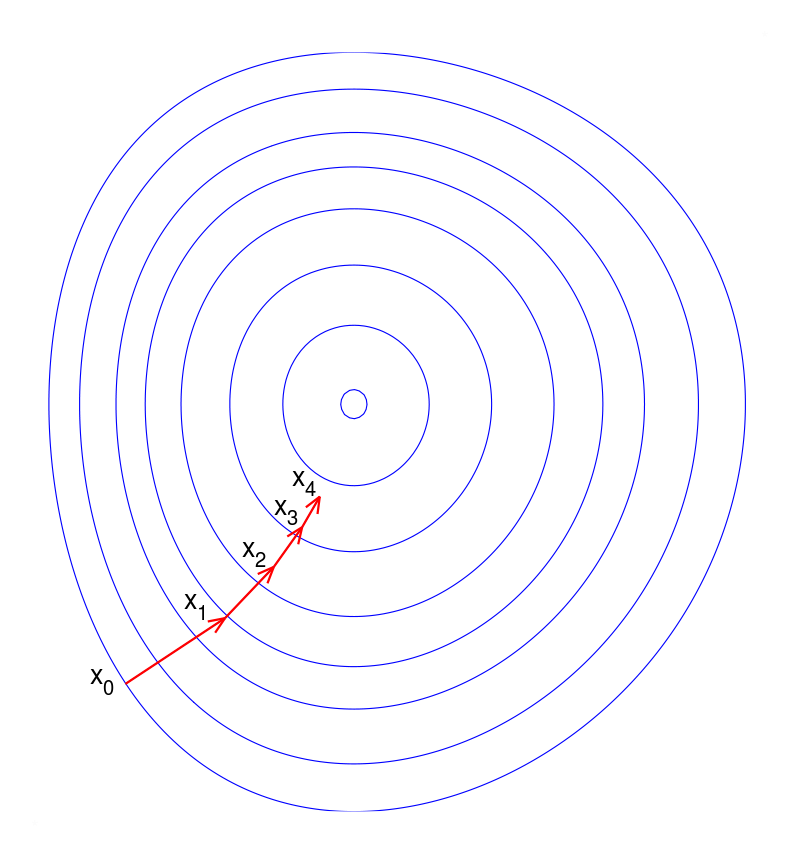
\includegraphics[width=0.6\textwidth]{images/Training (teoria)/Gradient descend.png}
    \caption{Illustration of the gradient method on level sets, the learning rate is updated at each iteration.\cite{wiki:gradientDescend}}
    \label{gradientDescentImage}
\end{figure}



\subsection{Stochastic gradient descent \cite{bottou2012stochastic}}
The method of \textbf{stochastic gradient descent}, unlike the gradient method, performs an update for each $Q_i$\footnote{In the case where the $Q$ is written as a sum of terms that each depend only on one element of the dataset, it implies that the method performs an update for each element of the dataset}. It has the form:
\begin{align*}
    &\text{Given an initial value }\omega_0, \eta_0\\
    &\text{To be repeated until an approximation of the minimum is found:}\\
    &\quad\text{Mixing the dataset}\\
    &\quad\text{For }i=1,...,n:\\
    &\quad\quad\omega_{k+1}=\omega_k -\eta_k\cdot \nabla Q_i(\omega_k)
\end{align*}
Since we only have to calculate the gradient for one addend of $Q$ at a time, it is a much faster method, although these frequent updates cause a high fluctuation of the objective function, as can be seen from the figure \ref{MomentumMethod}.\\
Although fluctuation may seem a disadvantage of the method, it is precisely this that allows it to avoid local minima and tend towards better approximations. The gradient method seen above, on the other hand, converges to the minimum of the basin in which the initial data was chosen.\\
On the other hand, fluctuation complicates convergence to the exact minimum due to the frequent changes the function undergoes. However, it has been shown that when slowly decreasing the learning rate, the method shows the same convergence behaviour as the gradient method. 


\newpage
\subsection{Method of moments \cite{ruder_2022}}
The stochastic gradient method has difficulty traversing \textit{burrows}, i.e. areas where the surface curves more steeply in one dimension than another. In these scenarios, the method oscillates along the slopes of the gully, while it hesitantly progresses along the bottom towards the minimum, as shown in the figure \ref{MomentumMethod}.\\
The \textbf{momentum method} is a method that helps accelerate the stochastic gradient method in the desired direction and dampen oscillations, as seen in the figure \ref{MomentumMethod}. It has the form:

\begin{align*}
    &\text{Given an initial value }\omega_0, \eta_0, v_0=0\\
    &\text{To be repeated until an approximation of the minimum is found:}\\
    &\quad\text{Mix the dataset}\\
    &\quad\text{For }i=1,...,n:\\
    & \quad\quad v_t=\gamma v_{t-1}+\eta_k\cdot \nabla Q_i(\omega_k)\\
    &\quad\quad\omega_{k+1}=\omega_k - v_t
\end{align*}
The $\gamma$ term is called \textit{momentum} (or \textit{quantity of motion}) and is usually set to 0.9.\\
Basically what happens is analogous to when you push a ball down a hill: the ball accumulates momentum
as it rolls downhill getting faster and faster (until it reaches its terminal velocity, if there is
air resistance, i.e. $\gamma<1$). 
The same thing happens with parameter updates: in the vector, the "momentum" term favours the dimensions in which the gradient points in the same direction and disfavours the others. As a result, faster convergence and reduced oscillation is achieved, reducing the problems of the stochastic gradient method, as shown in figure \ref{MomentumMethod}.

\begin{figure}[h]
\centering
\begin{subfigure}{.5\textwidth}
  \centering
  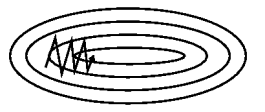
\includegraphics[width=\linewidth]{images/Training (teoria)/SGD Momentum a.PNG}
  \caption{Without momentum.}
\end{subfigure}%
\begin{subfigure}{.5\textwidth}
  \centering
  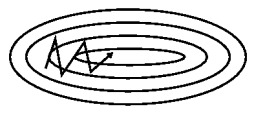
\includegraphics[width=\linewidth]{images/Training (teoria)/SGD Momentum b.PNG}
  \caption{With momentum.}
\end{subfigure}
\caption{Method of moments applied to the stochastic gradient method. \cite{ruder_2022}}
\label{MomentumMethod}
\end{figure}

\newpage
\subsection{AdaGrad \cite{JMLR:v12:duchi11a}}
The \textbf{AdaGrad} method (short for \textit{Adaptive Gradient algorithm}) is an optimisation algorithm based on the stochastic gradient method that uses an independent learning rate for each $\omega_i$. For $\omega_i$ terms that have a higher gradient or frequent updates, the method imposes a lower learning rate so as not to exceed the minimum. Conversely, those with a low gradient or infrequent updates will have a higher learning rate, so as to be trained quickly.\\



Adagrad improves the robustness of the stochastic gradient method and converges more quickly, especially when the data distribution is sparse; it has demonstrated excellent results in the training of large-scale neural networks (e.g. Google).

\begin{align*}
    &\text{Given an initial value }\omega_0, \eta\\
    &\text{To be repeated until an approximation of the minimum is found:}\\
    &\quad\text{Mix the dataset}\\
    &\quad\text{For }i=1,...,n:\\
    &\quad\quad \text{For each component $j$ of $\omega$:}\\
    &\quad\quad\quad g_{k,j}=(\nabla Q_i(\omega_k))_j\\
    &\quad\quad\quad\omega_{k+1,j}=\omega_{k,j} - \frac{\eta}{\sqrt{G_{k,j}}+\epsilon}g_{k,j}
\end{align*}
Where $G_{k,j}=\sum_{t=1}^{k}g_{t,j}^2$ and $\epsilon$ a small term to avoid division by zero (usually $10^{-8}$).\\
Since it adapts the learning rate, one of the main advantages of the method is that it eliminates the need to manually adjust $\eta_k$: generally $\eta=0.01$ is set.\\
The weak point of Adagrad is the accumulation of squared gradients in the denominator: as each added term is positive, the accumulated sum continues to grow during training. This causes the learning rate to decrease and tend to become infinitesimally small, at which point the algorithm is no longer able to acquire further knowledge.


\newpage
\subsection{Adam \cite{kingma_adam_2017}}\label{adam}
The \textbf{Adam} method (short for \textit{Adaptive Moment Estimation}) is, like the previous one, an adaptive learning rate method for each parameter. It derives from other methods (AdaDelta, RMSprop) that attempt to reduce the monotonically decreasing learning rate of the AdaGrad method. In fact: instead of accumulating all past gradients squared, the sum of the gradients is recursively defined as a decreasing average of all past quadratic gradients, which thus depends on the previous average and the current gradient, and is called $v_k$. Furthermore, Adam's method predicts the same decreasing average of past gradients, called $m_k$.


\begin{align*}
    &\text{Given an initial value }\omega_0, \eta, m_0=0, v_0=0\\
    &\text{To be repeated until an approximation of the minimum is found:}\\
    &\quad\text{Randomly shuffles the dataset}\\
    &\quad\text{For }i=1,...,n:\\
    &\quad\quad \text{For each $j$ component of $\omega$:}\\
    &\quad\quad\quad g_{k,j}=(\nabla Q_i(\omega_k))_j\\
    &\quad\quad\quad m_k=\beta_1m_{k-1}+(1-\beta_1)g_{k,j}\\
    &\quad\quad\quad v_k=\beta_2v_{k-1}+(1-\beta_2)g^2_{k,j}\\
    &\quad\quad\quad \hat{m}_k = \frac{m_k}{1-\beta_1^k}\\
    &\quad\quad\quad \hat{v}_k = \frac{v_k}{1-\beta_2^k}\\
    &\quad\quad\quad\omega_{k+1,j}=\omega_{k,j} - \frac{\eta}{\sqrt{\hat{v_k}}+\epsilon}\hat{m_k}
\end{align*}
The terms $m_k$ and $v_k$, the decreasing averages of the gradients and the square gradients, are estimates of the first moment and the second moment of the gradients, as defined in the method of moments. Since $m_k$ and $v_k$ are biased towards values close to zero, corrected $\hat{m}_k$ and $\hat{v}_k$ estimators are used. We generally impose values $\beta_1=0.9$ and $\beta_2=0.999$.

\newpage
Figure \ref{comparison} compares a number of methods in cost function minimisation in a neural network. It can be seen that Adam's method is much more efficient than the other methods introduced in the paper.
\begin{figure}[h]
    \centering
    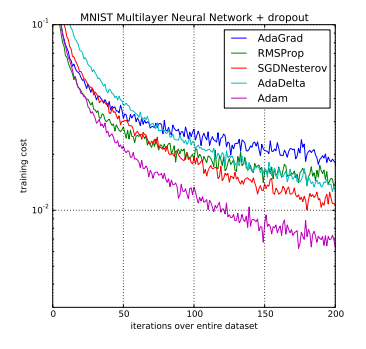
\includegraphics[width=0.75\textwidth]{images/Machine learning/Comparison.PNG}
    \caption{Comparison of methods for minimising a cost function in a neural network. \cite{kingma_adam_2017}}
    \label{comparison}
\end{figure}